\PassOptionsToPackage{dvipsnames}{xcolor}
\documentclass[10pt,externalviewer]{beamer}

\usepackage[dvipsnames]{xcolor}
\usepackage{amssymb}
\usepackage{rotating}
\usepackage{amsmath}
\usepackage{hyperref}
\usepackage{bookmark}
\usepackage{bigints}
\usepackage{graphics}
\usepackage{natbib}
\usepackage{relsize}
\usepackage{caption}
\usepackage{subcaption}
\usepackage{framed}
\usepackage{tikz}
\usepackage{lipsum}
\usepackage[italian]{babel}
\usepackage[utf8]{inputenc}
\usepackage[T1]{fontenc}
\usepackage[mode=math]{siunitx}
\usepackage[absolute,overlay]{textpos}
\usepackage{pdfcolparallel}
\usepackage{tcolorbox}
\usepackage{physics}
\usetikzlibrary{decorations.pathreplacing}
\tcbuselibrary{fitting}

\renewcommand{\arraystretch}{2}

\makeatletter
\newcommand\xleftrightarrow[2][]{
  \ext@arrow 9999{\longleftrightarrowfill@}{#1}{#2}}
\newcommand\longleftrightarrowfill@{
  \arrowfill@\leftarrow\relbar\rightarrow}
\makeatother

\definecolor{PDred}{HTML}{9B0014}

\mode<presentation>
{
  \usetheme{Warsaw}
 %\usetheme{Madrid}
 %\usetheme{Montpellier}
 %\usetheme{Marburg} 
  \usecolortheme[named=PDred]{structure}
  \setbeamercolor{alerted text}{fg=PDred}
  \setbeamercovered{transparent}
  \setbeamertemplate{section in toc}[ball unnumbered]
  \usefonttheme[]{serif}
  \setbeamerfont{author}
  {size=\scriptsize,parent=structure}
  \setbeamerfont{date}
  {parent=structure}
  \setbeamerfont{title}
  {size=\Large,parent=structure}
  \setbeamerfont{sectiontitle}
  {size=\Large,parent=structure}
  \setbeamerfont{short title}
  {size=\tiny}
}

%\setbeamertemplate{footline}{\hfill\insertframenumber/\inserttotalframenumber} 

\expandafter\def\expandafter\insertshorttitle\expandafter{%
  \insertframenumber\,/\,\inserttotalframenumber}

\newcommand{\backupbegin}{
   \newcounter{framenumberappendix}
   \setcounter{framenumberappendix}{\value{framenumber}}
}
\newcommand{\backupend}{
   \addtocounter{framenumberappendix}{-\value{framenumber}}
   \addtocounter{framenumber}{\value{framenumberappendix}} 
}

\newcommand{\refer}[1]{%
   \begin{flushright}
      {\alert{\tiny #1}}
   \end{flushright}}
  
\newcommand{\lrefer}[1]{%
   \begin{flushleft}
      {\alert{\tiny #1}}
   \end{flushleft}}
  
\newcommand{\param}[1]{%
   \begin{flushright}
      {\small #1}
   \end{flushright}
   \vspace{-1.5\baselineskip}
}

%\newcommand{\sech}{\mathop{\rm sech}\nolimits}
\newcommand{\sgn}{\mathop{\rm sgn}\nolimits}
\newcommand{\etal}{{\em et al.}}


\title{Simulation and Analysis of 1D Wave Propagation under Various Physical Models}

\author[Dario Liotta]{\large{\textbf{Dario Liotta}}}

\institute[Physics of Data (UniPD)]{
\begin{minipage}[c]{3.4truecm}

\includegraphics[width=\textwidth]{logo-unipd}
\end{minipage}
\begin{minipage}[c]{2truecm}
   \begin{flushleft}
   \end{flushleft}
\end{minipage}
\begin{minipage}[c]{4.2truecm}

\includegraphics[width=\textwidth]{logo-dfa}
\end{minipage}}

\date{September 6th 2025 \\ Course of \textbf{Quantum Information and Computing} \\ Academic Year 2024/2025}

\begin{document}

\begin{frame}[plain]
\titlepage
\end{frame}

\section{Finite Element Method}

\begin{frame}
   \frametitle{Numerical methods for differential equations}

   \begin{figure}
    \centering
    \begin{tikzpicture}[x=0.89cm]

        \node[align=left] at (0,5) (A) {\underline{\small{\textbf{\textcolor{BrickRed}{O}}}\footnotesize{rdinary }\small{\textbf{\textcolor{BrickRed}{D}}}\footnotesize{ifferential }\small{\textbf{\textcolor{BrickRed}{E}}}\footnotesize{quations}}};

        \node at (0,3.8) (B) {\scriptsize{Crank-Nicolson Method}};

        \node at (-3.75,3.8) (C) {\scriptsize{Euler Method}};

        \node at (3.75,3.8) (D) {\scriptsize{Trotter-Suzuki Formula}};

        \draw[->] (A) -- (B);
        \draw[->] (0,4.5) -- (-3.75,4.5) -- (C);
        \draw[->] (0,4.5) -- (3.75,4.5) -- (D);

        \draw[decorate, decoration={brace, amplitude=8pt, raise=2pt}] (1.7,3.6) -- (-4.8,3.6);
        \node at (-1.55,3) (E) {\footnotesize{\textbf{\textcolor{BrickRed}{R}}}\scriptsize{unge-}\footnotesize{\textbf{\textcolor{BrickRed}{K}}}\scriptsize{utta}};

         

        \draw[BrickRed] (-6,2.5) -- (6,2.5);



        \node[align=left] at (0,2) (F) {\underline{\small{\textbf{\textcolor{BrickRed}{P}}}\footnotesize{artial }\small{\textbf{\textcolor{BrickRed}{D}}}\footnotesize{ifferential }\small{\textbf{\textcolor{BrickRed}{E}}}\footnotesize{quations}}};

        \node[align=left] at (0,0.4) (G) {\footnotesize{\textbf{\textcolor{BrickRed}{F}}}\scriptsize{inite}\\\footnotesize{\textbf{\textcolor{BrickRed}{V}}}\scriptsize{olume}\\\footnotesize{\textbf{\textcolor{BrickRed}{M}}}\scriptsize{ethod}};

        \node[align=left] at (-3.75,0.4) (H) {\footnotesize{\textbf{\textcolor{BrickRed}{F}}}\scriptsize{inite}\\\footnotesize{\textbf{\textcolor{BrickRed}{D}}}\scriptsize{ifference}\\\footnotesize{\textbf{\textcolor{BrickRed}{M}}}\scriptsize{ethod}};

        \node at (3.75,0.8) (I) {\scriptsize{Galerkin methods}};

        \node at (2.25,-0.3) (J) {\scriptsize{Spectral Method}};

        \node<1>[align=left] at (5.25,-0.69) (Ktext) {\footnotesize{\textbf{\textcolor{BrickRed}{F}}}\scriptsize{\textcolor{black}{inite}}\\\footnotesize{\textbf{\textcolor{BrickRed}{E}}}\scriptsize{\textcolor{black}{lement}}\\\footnotesize{\textbf{\textcolor{BrickRed}{M}}}\scriptsize{\textcolor{black}{ethod}}};

        \node<2->[draw,BrickRed,align=left] at (5.25,-0.69) (K) {\footnotesize{\textbf{\textcolor{BrickRed}{F}}}\scriptsize{\textcolor{black}{inite}}\\\footnotesize{\textbf{\textcolor{BrickRed}{E}}}\scriptsize{\textcolor{black}{lement}}\\\footnotesize{\textbf{\textcolor{BrickRed}{M}}}\scriptsize{\textcolor{black}{ethod}}};

        \draw[->] (F) -- (G);
        \draw[->] (0,1.5) -- (-3.75,1.5) -- (H);
        \draw[->] (0,1.5) -- (3.75,1.5) -- (I);
        \draw[->] (I) -- (3.75,0.3) -- (2.25,0.3) -- (J);
        \draw[->] (I) -- (3.75,0.3) -- (5.25,0.3) -- (Ktext);



        \draw[white] (0,-1.6) -- (0,-1.5);
    \end{tikzpicture}
\end{figure}
\end{frame}

\begin{frame}{Introduction to the problem}
   Solving a \textbf{\textcolor{BrickRed}{PDE}} means to find a function $u$ such that

   \begin{equation*}
      \mathcal{L}u=f
   \end{equation*}

   where $\mathcal{L}$ is a \underline{differential operator} and $f$ is a \underline{source term}.

   \vspace{0.3cm}

   The equation holds in a domain $\Omega$ and is completed by prescribing \textbf{boundary conditions} on $\partial\Omega$.

   \vfill

   \pause

   \begin{figure}[H]
    \centering
    \begin{tikzpicture}
        \node[align=center,text width=3.5cm] at (0,0) (A) {In most physical applications $\mathcal{L}$ is a \textcolor{BrickRed}{\underline{second-order} operator}};

        \node at (5,0) (B) {\footnotesize{\textbf{Heat} equation: $\mathcal{L}=\frac{\partial}{\partial t}-\textcolor{BrickRed}{\Delta}$}};

        \node at (4.965,1) (C) {\footnotesize{\textbf{Poisson} equation: $\mathcal{L}=-\textcolor{BrickRed}{\Delta}$}};

        \node at (5.25,-1) (D) {\footnotesize{\textbf{Wave} equation: $\mathcal{L}=\frac{\partial^2}{\partial t^2}-c^2\textcolor{BrickRed}{\Delta}$}};

        \draw[->] (A) -- (B);
        \draw[->] (2.25,0) -- (2.25,1) -- (C);
        \draw[->] (2.25,0) -- (2.25,-1) -- (D); 
    \end{tikzpicture}
\end{figure}
\end{frame}

\begin{frame}{Weak formulation}
   Galerkin methods rely on a \textbf{\textcolor{BrickRed}{weak formulation}}

   \vspace{0.5cm}

   \pause

   \begin{itemize}
      \item \underline{Multiply} by a \textcolor{BrickRed}{test function} $v$ and \underline{integrate} over the entire domain
      
      \begin{equation*}
         -\int_\Omega(\Delta u)vd\Omega=\int_\Omega fvd\Omega
      \end{equation*}

      \pause

      \item \underline{Integrate by parts} the left hand side
      
      \begin{equation*}
         -\int_\Omega(\Delta u)vd\Omega=\int_\Omega\nabla u\cdot\nabla vd\Omega-\int_{\partial\Omega}\frac{\partial u}{\partial n}vds
      \end{equation*}

      \pause

      \item \underline{Substitute} and get the new expression
      
      \begin{equation*}
         \int_\Omega\nabla u\cdot\nabla vd\Omega=\int_\Omega fvd\Omega+\int_{\partial\Omega}\frac{\partial u}{\partial n}vds
      \end{equation*}
   \end{itemize}
\end{frame}

\begin{frame}{About the test function}
   \begin{center}
      \begin{framed}
         The test function $v$ is introduced to check whether the PDE is satisfied \textit{\underline{on average}} throughout the domain.
      \end{framed}
   \end{center}

   \pause

   The problem becomes to find $u$ such that

   \begin{equation*}
      a(u,v)=F(v) \qquad \forall v\in V
   \end{equation*}

   where

   \begin{alignat*}{2}
      a(u,v)&=\int_\Omega\nabla u\cdot\nabla vd\Omega \qquad &&\text{is a \underline{bilinear form}}\\
      F(v)&=\int_\Omega fvd\Omega+\int_{\partial\Omega}\frac{\partial u}{\partial n}vds \qquad &&\text{is a \underline{linear functional}}
   \end{alignat*}
\end{frame}

\begin{frame}{Benefits of the weak formulation}
   \begin{table}[H]
    \centering
    \begin{tabular}{c c}
        \textbf{Strong formulation} & \textbf{Weak formulation}\\
        \hline
        $u\in C^2(\Omega)$ & $u,v\in H^1(\Omega)^{\boldsymbol{\textcolor{BrickRed}{\ast}}}$\\
        Holds pointwise in $\Omega$ & Holds on average on $\Omega$\\
        Derivatives exist classically & \renewcommand{\arraystretch}{0.8} \begin{tabular}{@{}c@{}}Derivatives exist in the \\ distributional sense\end{tabular}\\
        \textcolor{white}{Derivatives exist classicallyyyy} & \textcolor{white}{Derivatives exist classicallyyyy}
    \end{tabular}
\end{table}

   \vspace{-0.5cm}

   \uncover<2->{\begin{center}
      \begin{framed}
         In short: weak formulation requires \textbf{\textcolor{BrickRed}{less regularity}}
      \end{framed}
   \end{center}}

   \vspace{0.6cm}

   $^{\boldsymbol{\textcolor{BrickRed}{\ast}}}$\scriptsize{$H^1(\Omega)$ is a \textbf{Sobolev space} of functions with square-integrable first derivatives:}

   \begin{equation*}
      w\in H^1(\Omega)=\left\{w\in L^2(\Omega)\mid\nabla w\in L^2(\Omega)^d\right\}
   \end{equation*}

   \normalsize
\end{frame}

\begin{frame}{On boundary conditions}
   Another difference lies in the boundary condition prescription.

   \vspace{0.35cm}

   \pause

   \begin{figure}[H]
    \begin{tikzpicture}

        \small

        \node at (0,0) (A) {In strong formulation};
        \node at (4,0.5) (B) {\underline{\textbf{Dirichlet}}:};
        \node at (4.07,-0.5) (C) {\underline{\textbf{Neumann}}:};

        \node at (5.68,0.5) () {$u=g$};
        \node at (5.58,-0.5) () {$\frac{\partial u}{\partial n}=h$};

        \node at (6.88,0.58) () {on $\partial\Omega$};
        \node at (6.88,-0.48) () {on $\partial\Omega$};

        \draw[->] (A) -- (2.05,0) -- (2.05,0.5) -- (B);
        \draw[->] (2.05,0) -- (2.05,-0.5) -- (C);

        \normalsize
    \end{tikzpicture}
\end{figure}

   \vspace{-0.5cm}

   \pause

   \begin{figure}[H]
    \centering
    \begin{tikzpicture}
        \small

        \node at (0,5) (A) {In weak formulation};

        \footnotesize

        \node[align=center] at (-2.874,3.75) (B) {Dirichlet becomes\\ \textbf{\textcolor{BrickRed}{essential condition}}};
        \node[align=center] at (2.874,3.75) (C) {Neumann becomes\\ \textbf{\textcolor{BrickRed}{natural condition}}};

        \scriptsize

        \node[align=center,text width=4.86cm] at (-2.874,2.65) (D) {$\boldsymbol{v=0}$ on $\partial\Omega$ $\Rightarrow$ cancels boundary term\\ (no information available on $\frac{\partial u}{\partial n}$)};

        \node[align=center,text width=4.86cm] at (-2.874,1.65) (E) {$\boldsymbol{u=g}$ enforced on $\partial\Omega$ (final solution)};

        \node[align=center,text width=5cm] at (2.874,2.65) (F) {$\boldsymbol{v}$ \textbf{free} on $\partial\Omega$};

        \node[align=center,text width=5cm] at (2.874,1.65) (G) {$\boldsymbol{\frac{\partial u}{\partial n}=h}$ naturally enters weak form};

        \draw[->] (A) -- (-2.874,5) -- (B);
        \draw[->] (A) -- (2.874,5) -- (C);

        \normalsize
    \end{tikzpicture}
\end{figure}
\end{frame}

\begin{frame}{Shape functions}
   Galerkin methods allow to find an \underline{approximate solution}
   
   \begin{equation*}
      u_h\in V_h\subset H^1(\Omega) \qquad \text{where } V_h \ \text{is a \textbf{finite-dimensional} space} 
   \end{equation*}

   In this framework, the goal is to find $u_h$ such that

   \begin{equation*}
      \boxed{a\left(u_h,v_h\right)=F\left(v_h\right) \qquad \forall v_h\in V_h}
   \end{equation*}

   \vfill

   \pause

   A \textbf{basis of function} $\left\{\phi_i\right\}$ is chosen to express $u_h$ and to use it as \underline{test}:

   \begin{equation*}
      u_h=\sum_{j=1}^Nu_j\phi_j \ \Longrightarrow \ a\left(\sum_{j=1}^Nu_j\phi_j,\phi_i\right)=F\left(\phi_i\right) \qquad \forall i=1,\dots,N
   \end{equation*}

   \vfill

   \pause

   \begin{center}
      Functions $\phi_i$ model the solution $\longrightarrow$ \textbf{\textcolor{BrickRed}{shape functions}}
   \end{center}
\end{frame}

\begin{frame}{Mesh discretization}
   \begin{center}
      \begin{framed}
         \textbf{FEM} approach consists in the subdivision of the domain in a so-called \textbf{\textcolor{BrickRed}{mesh}}
      \end{framed}
   \end{center}

   \pause

   This choice brings several advantages:

   \begin{itemize}
      \item Good approximation of \textbf{complex geometries}
      \item Better capture of \textbf{local effects}
      \item Possibility of \textbf{adaptive refinement}
      \item Natural construction of a \textbf{global solution}
   \end{itemize}

   \visible<2>{\begin{figure}[H]
      \centering
      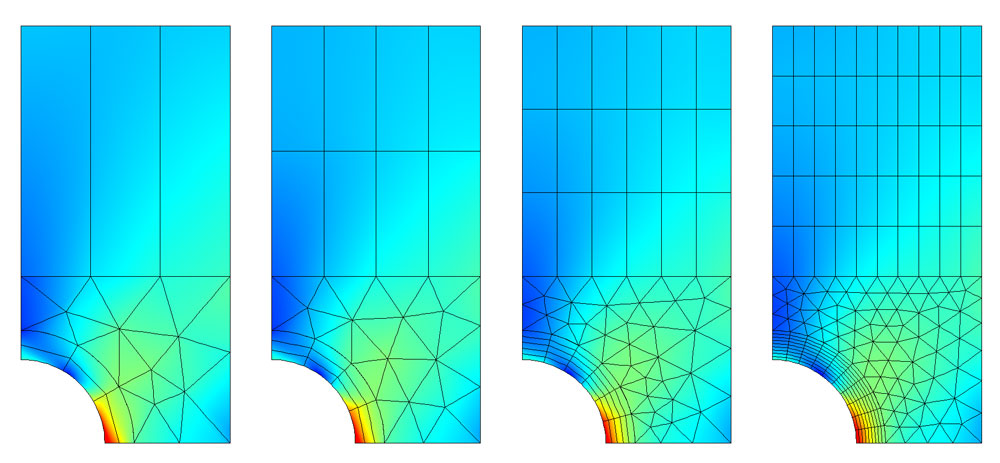
\includegraphics[width=0.72\textwidth]{Immagini/mesh-example.jpeg}
   \end{figure}}
\end{frame}

\begin{frame}{Elements}
   \begin{figure}[H]
      \centering
      \begin{tikzpicture}
         \small

         \node at (0,2) (A) {Discretization in different dimensions};
         \node at (-4,1) (B) {1D};
         \node at (0,1) (C) {2D};
         \node at (4,1) (D) {3D};

         \draw[->] (A) -- (C);
         \draw[->] (A) -- (-4,2) -- (B);
         \draw[->] (A) -- (4,2) -- (D);
      \end{tikzpicture}
   \end{figure}
\end{frame}

\begin{frame}{Application examples}

\end{frame}

\begin{frame}{Title}
   In \textcolor{BrickRed}{F}inite \textcolor{BrickRed}{E}lement \textcolor{BrickRed}{M}ethod, $V_h$ is generated by \textbf{local basis functions} with \underline{compact support}. Usually, one discretizes the domain using a so-called mesh
\end{frame}

\end{document}